\documentclass[12pt]{article}
\usepackage{epsfig}
\usepackage{graphicx}
\usepackage{color}
\usepackage[frenchb]{babel}
\usepackage{subfigure}
\usepackage{algorithm}
\usepackage{algpseudocode}
\usepackage{amsmath}
\usepackage{url}
\usepackage{listings}


% Pour pouvoir utiliser les accents directement dans LaTeX, sans utiliser les commandes \'
%\usepackage[latin1]{inputenc} % entree 8 bits iso-latin1
\usepackage[utf8]{inputenc} % entree 8 bits utf8, fonctionne avec MikTeX sur Windows.
\usepackage[T1]{fontenc}      % encodage 8 bits des fontes utilisees

% Pour agrandir les marges
\addtolength{\oddsidemargin}{-.875in}
\addtolength{\evensidemargin}{-.875in}
\addtolength{\textwidth}{1.75in}
\addtolength{\topmargin}{-.875in}
\addtolength{\textheight}{1.75in}

\makeatletter\renewcommand{\ALG@name}{Algorithme}


\begin{document}
\title{GLO-4001 Introduction à la robotique mobile \\  TP1 \\ 23 octobre 2017}
\author{Alexandra Mercier et Alexandre Gingras-Courchesne}
\maketitle


{\bf Attention! N'oubliez pas d'attacher le code de toutes les questions dans la remise .zip de votre travail. Si les codes sont manquants, nous pourrons retirer jusqu'à 20\% de la note. }

Pour tous les étudiants, vous devez fournir un rapport en un seul document (format pdf) et les fichiers matlab ou Python zippé. Pour toutes les questions, n'oubliez pas de mettre le détail des calculs.

% ================== Carte =======================
\section{Carte 2D à partir d'un gyroscope et d'un capteur de distance (15 pts)}

\subsection{Carte 2D locale (5 pts)}
\label{CarteLocale}

\subsubsection{Calculs}
Pour pouvoir créer un nuage de point sur un plan 2D, il faut utiliser nos données pour obtenir une variété de points x, y.
Pour cela, il faut:
\begin{enumerate}
        \item Convertir la tension de notre capteur en distance.
        \item Convertir la vitesse angulaire du gyroscope en angle.
        \item Obtenir un point (x, y) avec la distance et l'angle.
\end{enumerate}

\textbf{Convertir la tension du capteur}
Soit la fonction du capteur avant bruit:
\[ z(d) = 1/d \]

Comme le capteur est bruité, il faut consid\'erer celui-ci. On mod\'elise donc la fonction avec une gaussienne:

\textbf{Convertir la vitesse angulaire}
Soit :
\[ \frac{d\theta}{dt} = g \] o\`u g est la vitesse angulaire.
On peut approximer cela \`a:
\[ \frac{\Delta \theta}{\Delta t}  = g\]
Avec le temps t noté, on peut trouver la valeur de $\theta$ en ajoutant $\Delta t * g $ ou $ (t_{valeur précédente} - t_{valeur courante}) * g$.

Toutefois, cette technique va cumuler de l'erreur avec le temps.
Pour Réduire l'erreur du à l'intégration:

\textbf{Obtenir un point (x, y)}

Soit avec la trigonométrie:
\[ x = d*\cos(\theta) \] \[ y = d*\sin(\theta) \]

\subsubsection{Code}
Le fichier question1.py contient le code utilisé pour former la carte 2D.
\subsubsection{Carte}

\begin{figure}[ht]
 \begin{center}
  \begin{tabular}{c}
    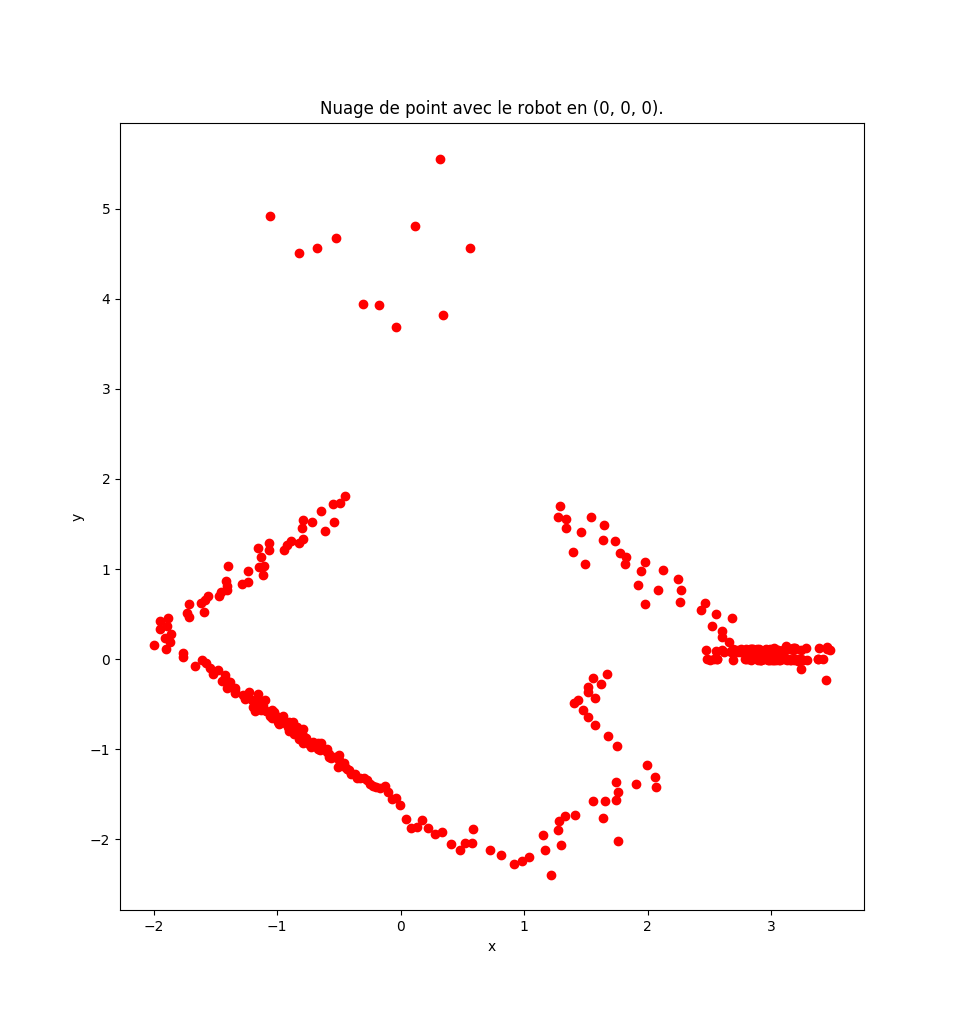
\includegraphics[width=0.75\textwidth]{q1-carte-local.png}
  \end{tabular}
 \end{center}
\vspace{-0.25in}
 \caption{Carte 2D générée avec les données matlab et le code python.}
    \label{carte-2d-locale}
\end{figure}

La figure \ref{carte-2d-locale} représente le nuage de point.

\newpage
\subsection{Localisation du robot dans la carte globale (10 pts)}

\subsubsection{Calculs}
\textbf{Création de $P_{Homogene}$:}

\[ \text{Soit } P_{Homogene} =
\begin{bmatrix}
    x_1 & x_2 & x_3 & ... & x_n \\
    y_1 & y_2 & y_3 & ... & y_n \\
    1   & 1   & 1   & ... & 1   \\
\end{bmatrix}
\]

\textbf{D\'etermination des matrices de transformation T:}

Soit pour faire une translation $[T_x, T_y]$, il faut multiplier $P_{Homogene}$ par la matrice

\[
    T =
    \begin{bmatrix}
        1 & 0 & T_{x} \\
        0 & 1 & T_{y} \\
        0 & 0 & 1
    \end{bmatrix}
    \]

\textbf{D\'etermination des matrices de transformation R:}

Soit pour faire une rotation de $\theta rad$, cela \'equivaut \`a multiplier par la matrice
\[
    R =
    \begin{bmatrix}
        \cos{\theta} & -\sin{\theta} & 0 \\
        \sin{\theta} & \cos{\theta} & 0 \\
        0 & 0 & 1 \\
    \end{bmatrix}
    \]

\subsubsection{Code}

Le code est disponible dans le fichier question1.py

\subsubsection{Réponse}

$T_x = 10$ et $T_y = 1.7$
$\theta = \frac{\pi}{4}$

\begin{figure}[ht]
 \begin{center}
  \begin{tabular}{c}
    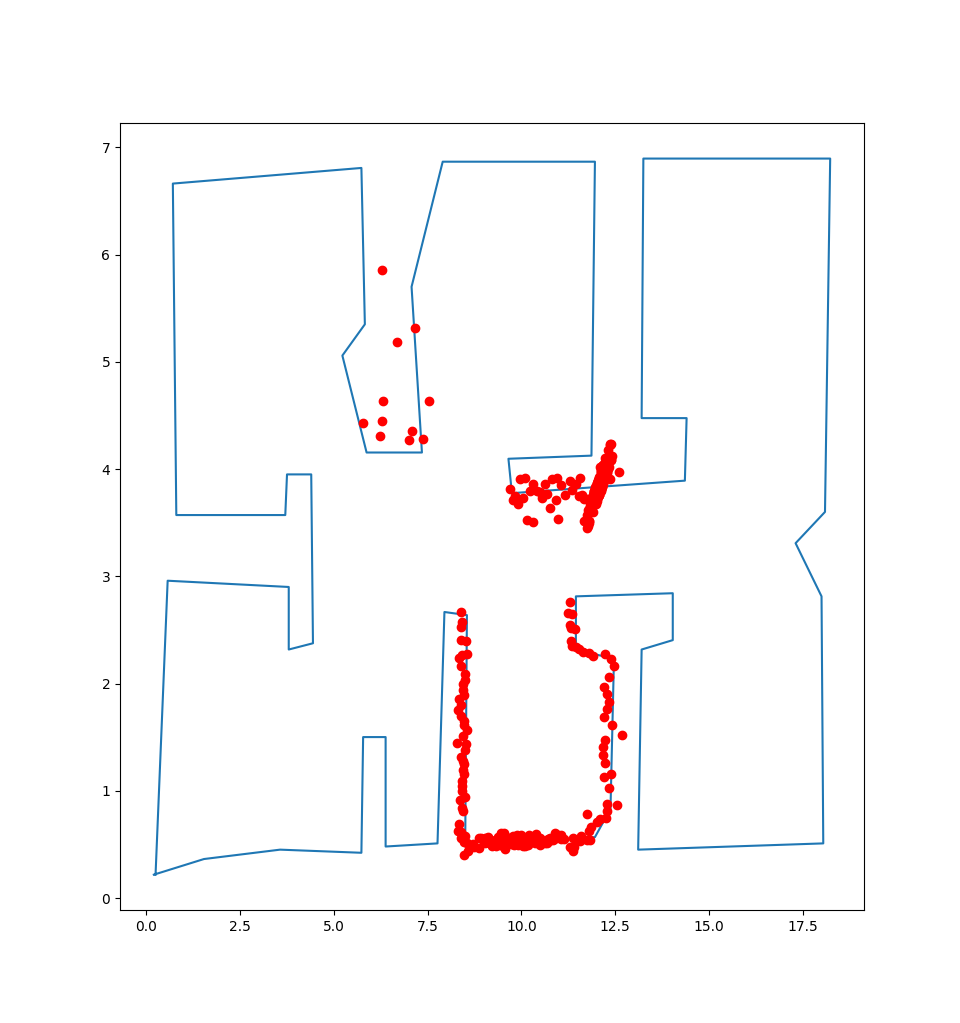
\includegraphics[width=0.75\textwidth]{q1-carte-nuage-superpose.png}
  \end{tabular}
 \end{center}
\vspace{-0.25in}
 \caption{Carte 2D fournit avec PGlobal superpos\'e}
    \label{carte-pglobal}
\end{figure}

La figure \ref{carte-pglobal} montre la carte réelle avec la matrice $P_{gloal}$ superposée.

% ================== CAMERA =======================
\newpage
\section{Modèle de caméra et positionnement par caméra}

\subsection{Génération d'une image (5 pts)}
\label{generation_image}
\subsubsection{Calculs}
Soit la relation entre le point correspondant [u, v] et la position dans le monde r\'eel $ [L_{ix}, L_{iy}, L_{iz}] $
\[ \left[ {\begin{array}{c}
                u \\
    v \\ \end{array} } \right] =
    \frac{f}{L_{iz}}
    \left[ {\begin{array}{c} L_{ix} \\ L_{iy} \\ \end{array}} \right]
\]

Comme la valeur $L_y$ est nulle, nous obtenons:


\[ \left[ {\begin{array}{c}
                u \\
    v \\ \end{array} } \right] =
    \frac{f}{L_{iz}}
    \left[ {\begin{array}{c} L_{ix} \\ 0 \\ \end{array}} \right]
=
    \left[ {\begin{array}{c} \frac{f}{L_{iz}} * L_{ix} \\ \frac{f}{L_{iz}} * 0 \\ \end{array}} \right]
=
    \left[ {\begin{array}{c} \frac{f}{L_{iz}} * L_{ix} \\ 0 \\ \end{array}} \right]

\]

On peut ainsi en conclure que:
\[
    u =  \frac{f}{L_{iz}} * L_{ix}
\]
\[
    v = 0
\]
o\`u u et v sont en pixels, et f = 1200 pixels.

\subsubsection{Code}

Le fichier question2.py contient la fonction make\_image\_uv\_pose qui convertie la position de $L_i$ en une position d'écran $ [u, v] $.

\subsection{Estimation de la pose de la caméra à partir des angles $\alpha$ et $\beta$ (5 pts)}

\subsubsection{Calculs}
Soit une fois $\alpha$ et $\beta$ obtenues, il faut retrouver la postion de la cam\'era avec ceux-ci.
Pour ce faire, il faut retrouver les cercles qui sont d\'etermin\'ees par les angles $\alpha$ et $\beta$, ainsi que par la position des points de repères.
La position en x dans le monde r\'eel des points de rep\`eres peut \^etre obtenu \`a partir de leur position dns l'image $u$ en faisaint l'inverse des calculs notés précedemment.

Avec deux points $l_1$ et $l_2$, ainsi que l'angle entre les deux points sur le cercle $\alpha$, on peut trouver le centre c:
\[  \vec{c} = \vec{l_m} + \frac{1}{2\tan{\alpha}}
\begin{bmatrix}
    0 & -1 \\
    1 & 0 \\
\end{bmatrix} (\vec{l_1} - \vec{l_2})
\]

et le rayon r est la distance entre le centre et un des deux points.

Les cercles définis par les trois points sont ainsi obtenues.
Il faut maintenant calculer les point d'intersection entre ces deux cercles.

\begin{figure}[ht]
 \begin{center}
  \begin{tabular}{c}
    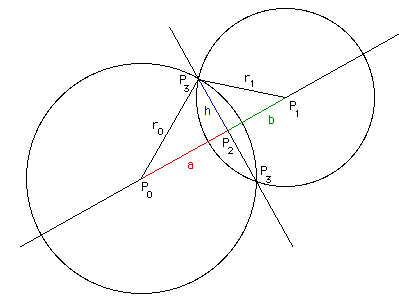
\includegraphics[width=0.55\textwidth]{circle_intersection.png}
  \end{tabular}
 \end{center}
\vspace{-0.25in}
 \caption{Intersection entre deux cercles}
    \label{circle_intersection}
\end{figure}

La figure \ref{circle_intersection} repr\'esente la relation math\'ematique pour obtenir l'intersection de deux cercles.
Cette image vient de \url{https://stackoverflow.com/questions/3349125/circle-circle-intersection-points}.

o\`u:

   \[ P_0 \text{ : Le centre du premier cercle} \]
   \[ r_0 \text{ : Le rayon du premier cercle} \]
   \[ P_1 \text{ : Le centre du deuxi\`eme cercle} \]
   \[ r_1 \text{ : Le rayon du deux\`eme cercle} \]


La distance entre les deux centres de cercles $d$ est:
\[ d = \sqrt{(P0_x - P1_x)^2 + (P0_y - P1_y)^2} \]
\[ a = \frac{r0^2 - r1^2 + d^2}{2 \cdot d} \]
\[ h = \sqrt{r0^2 - a^2} \]
\[ P2_x = P0_x + \frac{a(P1_x - P0_x)}{d} \]
\[ P2_y = P0_y + \frac{a(P1_y - P0_y)}{d} \]

Soit on obtient deux points d'intersection:

\[  p_{intersection1}x = P2_x + (h*(P1y - P0y))/d \]
\[  p_{intersection1}y = P2_y - (h*(P1x - P0x))/d \]

\[  p_{intersection2}x = P2_x - (h*(P1y - P0y))/d \]
\[  p_{intersection2}y = P2_y + (h*(P1x - P0x))/d \]

Un de ces deux points d'intersection est un de nos points de rep\`eres.
L'autre est la position de la cam\'era.

\subsubsection{Code}
La fonction alpha\_beta\_from\_three\_coordinates(f, c1, c2, c3) dans question2.py est le code qui a été utilisé en classe pour retrouver $\alpha$ et $\beta$.

La fonction circle\_from\_pts\_and\_angle(p1, p2, angle) dans question2.py est le code qui a été utilisé en classe pour retrouver les deux cercles correspondant \`a $\alpha$ et $\beta$.

La fonction get\_circle\_intersections(c0, r0, c1, r1) dans question2.py retourne les deux points d'intersection du cercle.
Un de ces deux points devrait \^etre environ la position d'un des points de rep\`eres.
L'autre est celui de la cam\'era.

Il y a un example de l'impl\'ementation dans le main de question2.py.

\subsubsection{Réponse}
Soit la caméra dans le plan 2d $ [x_{carte}, y_{carte}]$ est $[0.045, -0.084]$m. 

\subsection{Impact du bruit sur l'estimation des repères (10 pts)}
\subsubsection{Code}
La fonction loop\_question23(metres\_recule, ecart\_type) est ce qui est utilis\'e pour faire les calculs pour le nuage de points bruit\'es.

\subsubsection{Réponse}

\begin{figure}[ht]
 \begin{center}
  \begin{tabular}{c}
    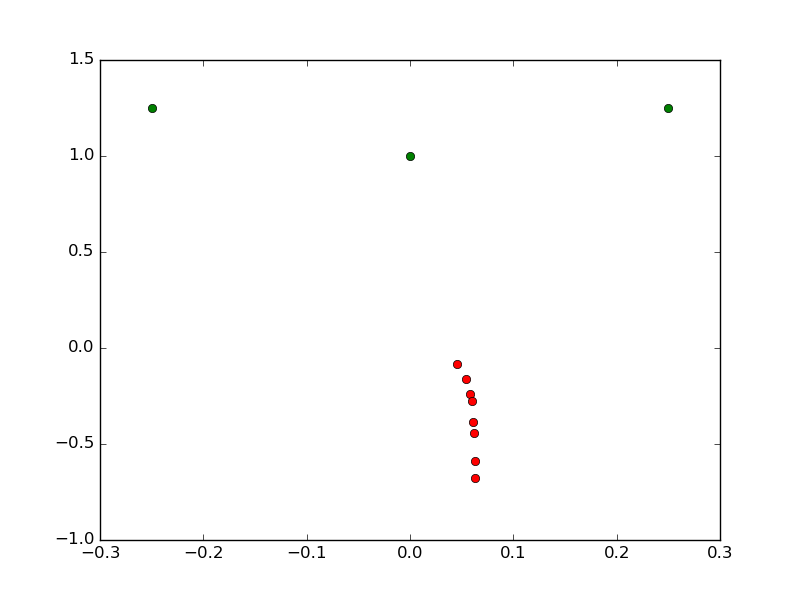
\includegraphics[width=0.55\textwidth]{../src/reponse-question-23.png}
  \end{tabular}
 \end{center}
\vspace{-0.25in}
    \caption{Position de la caméra estimé (en rouge) en relation avec la position des points de repère (en vert)}
    \label{impact-bruit-camera}
\end{figure}

% ================== STEREO =======================
\newpage
\section{Imagerie stéréo  (15 pts)}

\subsection{Distance focale $f$ (4 pts)}
\subsubsection{Calculs}
Pour obtenir f, il faut connaître les valeurs [u, v] de la tour verte.
Mesur\'ee avec une r\`egle, on obtient:
\[ u = 0 px \text{(centre de l'image)}\]
\[ v = 310 px\]
Sachant que:
\[ \text{Axe des v: } 0.7cm = 200px \]
En reprenant la fonction trouv\'ee en \ref{generation_image}, on sait que :

\[
    u =  \frac{f}{L_{iz}} * L_{ix}
\]
\[
    v =  \frac{f}{L_{iz}} * L_{iy}
\]
On isole $f$ dans l'\'equation de v:
\[
    f =  \frac{v * L_{iz}}{L_{iy}}
\]

Comme on sait que la tour fait 15cm de hauteur ($L_{iy} = 15$) et que celle-ci est \`a une distance de 95cm de la cam\'era ($L_{iz} = 95$):
\[
    f =  \frac{v * L_{iz}}{L_{iy}} = \frac{310px * 95 cm}{15cm} = 1963.33 px = 2000 px
\]


\subsubsection{Code}
\subsubsection{Réponse}
La distance focale est d'environ 2000 pixels.

\subsection{Estimation de la distance $A_z$ de chaque tour LEGO (6 pts)}
\label{estimation_distance_Az}
\subsubsection{Calculs}

\begin{table}[h]
\caption{Disparit\'e $d$ mesur\'ee avec la r\`egle}
\label{TableCoord}
\begin{center}
\begin{tabular}{|c|c|c|c|}
\hline
    tour   &  $u_{gauche}$  &  $u_{droite}$  &  $d$ $(u_g - u_d)$ \\
\hline
    rouge  & -1.75cm & -2.65cm & 0.90cm \\
    bleu   & 1.70cm & 0.50cm & 1.20cm \\
    jaune  & 2.50cm & 1.65cm & 0.85cm \\
\hline
\end{tabular}
\end{center}
\end{table}

Pour convertir la disparit\'e en pixels, on utilise la r\`egle de de trois sachant que:

\[ \text{Axe des u:} 1.2cm = 200px \]


\begin{table}[h]
\caption{Disparit\'e $d$ en pixels}
\label{TableCoord}
\begin{center}
\begin{tabular}{|c|c|c|c|}
\hline
    tour   &  $d$ \\
\hline
    rouge  &  150px \\
    bleu   &  200px \\
    jaune  &  140px \\
\hline
\end{tabular}
\end{center}
\end{table}

On peut trouver $A_z$ avec la formule:
\[ A_z = \frac{f \dot b}{d}\]
Avec f = 2000px et b = 5cm.

\subsubsection{Code}
\subsubsection{Réponse}

\begin{table}[h]
\caption{Distance en $z$ des centres des faces des colonnes.}
\label{TableCoord}
\begin{center}
\begin{tabular}{|c|c|}
\hline
 tour   & $A_z$ \\
\hline
 rouge  & 67cm \\
 bleu   & 50cm \\
jaune   & 71cm \\
\hline
\end{tabular}
\end{center}
\end{table}


\subsection{Estimation de la coordonnée $A_x$ de chaque tour LEGO (5 pts)}
\subsubsection{Calculs}
On r\'eutilise les valeurs de $u_{gauche}$ mesur\'ees en \ref{estimation_distance_Az}.
Puis, on les convertie en pixels.

\begin{table}[h]
    \caption{$u_{gauche}$ en pixels}
\label{TableCoord}
\begin{center}
\begin{tabular}{|c|c|}
\hline
    tour   &  $u_{gauche}$\\
\hline
    rouge  & -290px  \\
    bleu   & 280px   \\
    jaune  & 420px   \\
\hline
\end{tabular}
\end{center}
\end{table}

Avec la trigonométrie, on peut conlure que $u_{gauche} \propto A_x$ soit :
\[ u_g = \frac{f}{A_z}A_x\]
\[ A_x = \frac{u_g \dot A_z}{f} \]
Sachant que $f = 2000px$ et en utilisant les valeurs de $A_z$ trouvées en \ref{estimation_distance_Az}.

\subsubsection{Code}
\subsubsection{Réponse}

\begin{table}[h]
\caption{Coordonnée en $x$ des centres des faces des colonnes.}
\label{TableX}
\begin{center}
\begin{tabular}{|c|c|}
\hline
 tour   &  $A_x$ \\
\hline
 rouge  &  -9.7cm     \\
 vert   &  0.0cm   \\
 bleu   &  7.0cm    \\
 jaune  &  15cm     \\
\hline
\end{tabular}
\end{center}
\end{table}


% ==================  FAST =======================
\newpage
\section{Extracteur de coin FAST (13 pts)}
 \label{SectionFAST}

\subsection{Fonction d'extraction des coins FAST (7 pts)}
Le fichier fast.py contient la classe Fast, qui extrait les coins d'une image avec un centre et un threshold donn\'e.
\subsection{Test de votre fonction \texttt{DetectionCoinFAST} sur une image réelle (6 pts)}

\begin{figure}[ht]
 \begin{center}
  \begin{tabular}{c}
    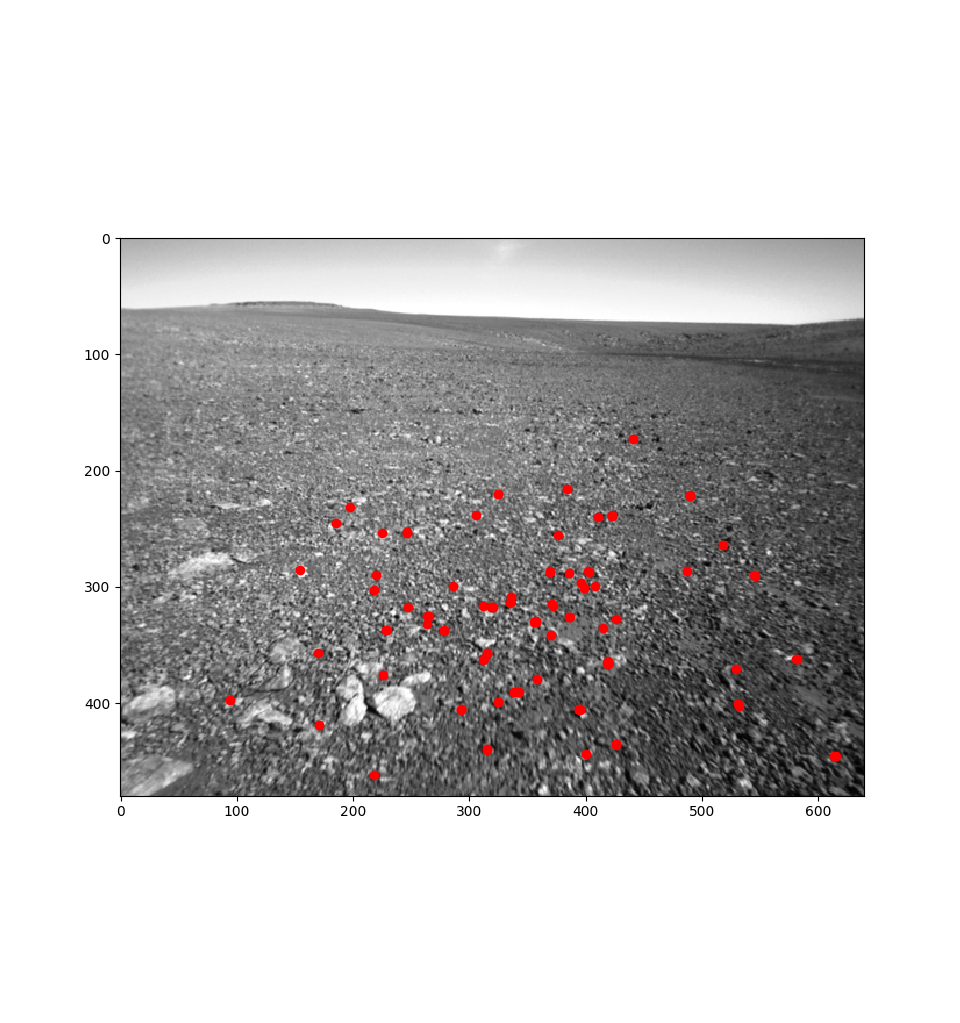
\includegraphics[width=0.55\textwidth]{q4-detection-keypoint.png}
  \end{tabular}
 \end{center}
\vspace{-0.25in}
 \caption{Coins d\'etect\'es avec un threshold de 100}
    \label{detection-coin-100}
\end{figure}

Environ 65 000 coins ont \'et\'e d\'etect\'es avec le treshold de 10.
Pour le threshold de 100, environ une cinquantaine de coins ont \'et\'e d\'etect\'es.

Avec le threshold de 100, les coins rep\'er\'es ont tendance \`a \^etre devant le robot, souvent pr\`es.
Moins de coins sont d\'etect\'es dans l'horizon.
% ================== Descripteur BRIEF =======================

\newpage
\section{Descripteur BRIEF (17 pts pour GLO-4001, 27 pts pour GLO-7021)}

\subsection{Fonction calculant un descripteur BRIEF (3 pts)}

\subsection{Appariement features image gauche-droite (5 pts)}
 Appliquez votre pipeline sur les images suivantes :
 \begin{itemize}
 \item \texttt{bw-rectified-left-022146small.png} et
 \item \texttt{bw-rectified-right-022146small.png},
 \end{itemize}
\end{document}
